\chapter{Der Detroit im aktuellen Zustand}

\section{Batterie}
Als Batterie für den Detroit sollten die modernen Lithium-Ionen-Akkumulatoren des Peugeot-Unfallfahrzeuges verwendet werden. Dabei mussten jedoch einige Anpassungen vorgenommen werden, da die Batterien zum einen nicht die selbe Spannung besassen, zum anderen beim Detroit auch zwei unabhängige Batterien verbaut waren. Dies zog umfangreiche Anpassungen mit sich, die nachfolgend erläutert werden.

\subsection{Funktion von Lithium-Ionen-Akkumulatoren} \label{kap_liion}

Lithium-Ionen-Akkumulatoren sind in der heutigen Zeit Standard. Das heisst in allen neuartigen Handys, Mobiltelefonen aber auch in Fahrzeugen werden diese verbaut und es wird immer mehr auf Blei-Akkus verzichtet. Die Technologie um die Lithium-Ionen Akkus ist jedoch im Vergleich zu Blei-Batterien sehr jung, genauer gesagt ca. 50 Jahre alt, und hinter den effizienten Akkus liegt eine aufwändige Ladetechnik. Nachfolgend wird kurz die Funktionsweise und die Lade-/Entladekurve der Lithium-Ionen-Akkus erläutert.

\paragraph{Aufbau/Grundfunktion}

Der Name Lithium-Ionen-Akkumulator kommt von den Lithiumionen die frei zwischen den beiden Elektroden wandern. Durch einen Separator sind die beiden Elektroden durch direkten Kontakt geschützt. Die positive Elektrode besteht aus Lithium-Metalloxide und die negative aus Graphit. Wichtig ist, dass die Elektrolytlösung frei von Wasser ist, damit es nicht mit dem Lithium reagiert.
Grundsätzlich funktioniert der Akku so, dass im Ladevorgang positiv geladene Lithiumionen von der positiven zur negativen Elektrode übergehen und an der Kathode hängen bleiben. Gleichzeitig liefert der Ladestrom die Elektronen über eine von aussen angelegte Verbindung. Beim Entladevorgang funktioniert wie beim Blei-Akku das umgekehrte. Die Elektronen fliessen über den äusseren Stromkreis zur positiven Elektrode. Der Aufbau und die Grundfunktion sind in Abbildung \ref{fig:liion_akku} dargestellt. \cite{liion_akku_aufbau_funktion2}

\begin{figure}[h!]
	\centering
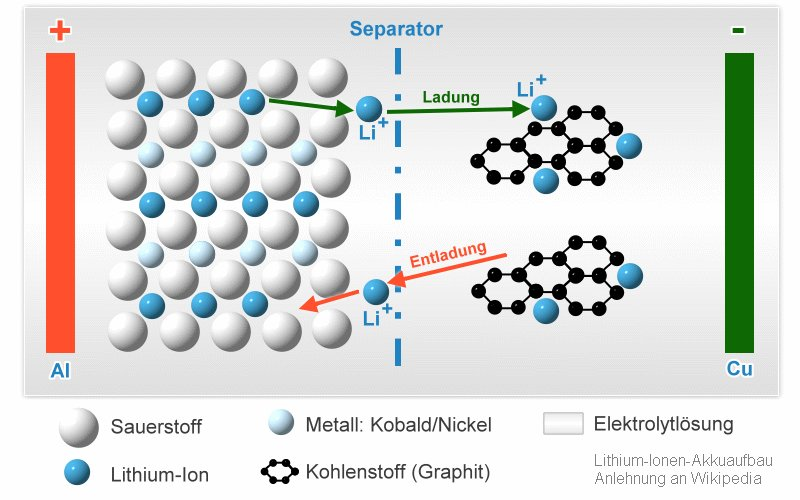
\includegraphics[width=0.75\textwidth]{images/aufbau_liion.jpg}
	\caption{Aufbau/Grundfunktion Lithium-Ionen-Akkumulator \cite{liion_akku_aufbau_funktion1}}
	\label{fig:liion_akku}
\end{figure}

\newpage

\paragraph{Lade-/Entladekurve}

Die typischen Lade-/Entladekurven sind nachfolgend in Abbildung \ref{fig:liion_akku_kurve} aufgeführt:

\begin{figure}[h!]
    \subfigure[Ladekurve \cite{liion_ladekurve}]
    {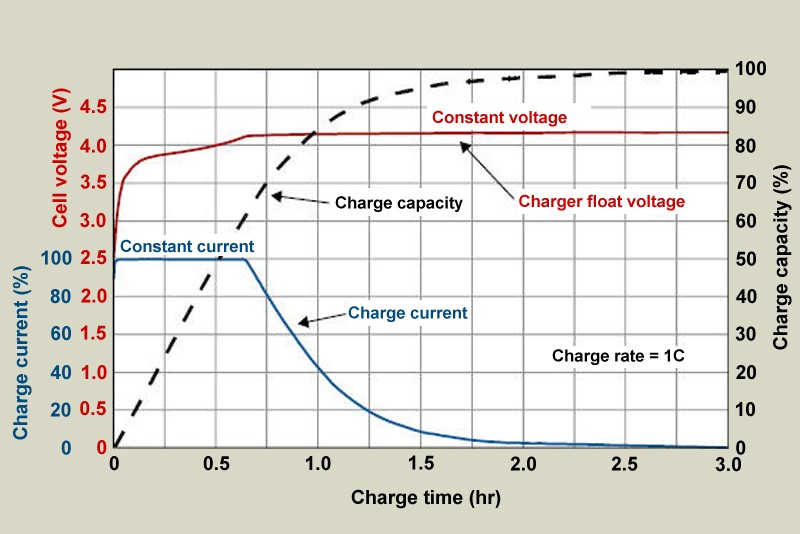
\includegraphics[width=0.49\textwidth]{images/liion_ladekurve.jpg}}
    \subfigure[Entladekurve \cite{liion_entladekurve}]
    {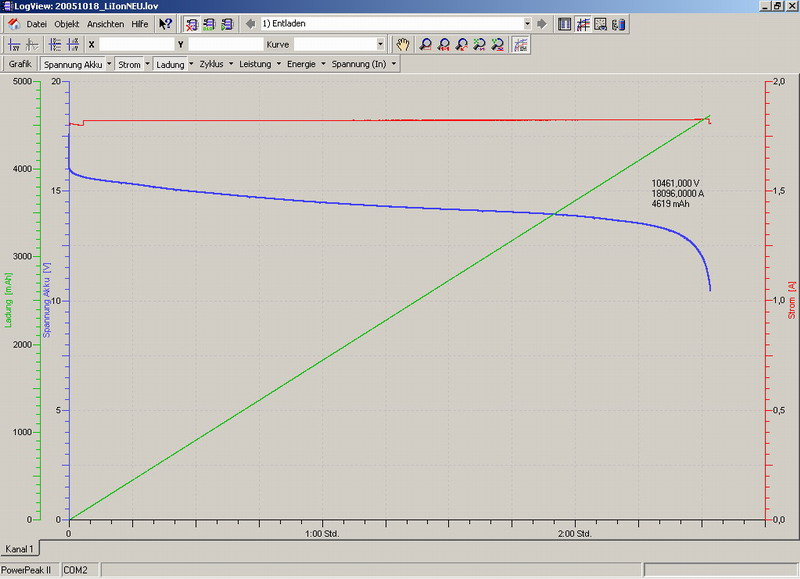
\includegraphics[width=0.49\textwidth]{images/liion_entladekurve.jpg}}
\caption{Lade-/Entladekurve Lithium-Ionen-Akkumulator}
\label{fig:liion_akku_kurve}
\end{figure}

Es ist zu sehen, dass die Batteriespannung innert kurzer Zeit stark ansteigt. Anschliessend ist die Steigung flacher jedoch einigermassen linear. Am Ende sinkt dann der Strom und die Spannung bleibt konstant bis 100\% der Kapazität erreicht wird.
Das nahezu selbe funktioniert beim Entladevorgang jedoch einfach umgekehrt. Die Spannung ist über einen weiten Zeitraum linear und erst am Ende bricht sie zusammen.
Zu erwähnen ist noch, dass es sich bei den beiden Figuren in Abbildung \ref{fig:liion_akku_kurve} um unterschiedliche Verschaltungen der Batterien handelt. Aus diesem Grund sind auch die Spannungen unterschiedlich, jedoch bleibt die Form der Kurven gleich.

\newpage

\subsection{Vergleich Blei / Lithium-Ionen} \label{kap:Vergleich_liion_pb}

Um die Unterschiede von Lithium-Ionen zu Blei-Akkus besser zu verstehen, sind nachfolgend kurz einige Vor- und Nachteile aufgelistet:

\paragraph{Vorteil Blei}

Kurzfristige Lieferung von hohen Strömen ist für Blei-Akkumulatoren kein Problem. Sie besitzen ein gutes Preis-/Leistungsverhältnis und sind sehr zuverlässig, wenn Wartung und Pflege eingehalten werden. Ebenfalls sind sie relativ einfach in der Ladetechnik.

\paragraph{Nachteil Blei}

Die Energiedichte ist sehr gering. Das heisst es braucht ein grosses Volumen und somit ein hohes Gewicht um überhaupt ansatzweise eine gute Kapazität zu erreichen. Auch ist das Elektrolyt säurehaltig, womit Verätzungsgefahr besteht. Zusätzlich können normale Blei-Akkus nur waagerecht gelagert oder verbaut werden, da sonst das gefährliche Elektrolyt auslaufen würde.

\paragraph{Vorteil Lithium-Ionen}

Der Akku besitzt eine sehr hohe Energiedichte, was auch für das geringe Gewicht der Akkumulatoren zuständig ist. Ebenfalls sind die Akkumulatoren sehr lange haltbar und müssen sehr selten ausgetauscht werden. Auch ist es möglich diese über Monate aufzubewahren ohne grosse Einbussen in der Kapazität zu bemerken.

\paragraph{Nachteil Lithium-Ionen}

Eine aufwändige Ladetechnik und Batteriemanagementsystem, kurz BMS, wird benötigt, da die Batterien sehr heikel gegenüber Über- und Unterspannung und auch Übertemperatur reagieren. Somit kommen immense Kosten hinzu.

\paragraph{Fazit}

Beide Akkutypen haben ihre Vor- und Nachteile und es kommt stark auf die Anwendung der Batterie an. Für Starterbatterien in einem normalen Auto kann ohne Probleme eine billige Blei-Batterie verwendet werden. Wenn jedoch wie in unserem Fall ein Fahrzeug nur mit Akkumulatoren läuft ist es sinnvoll auf das Gewicht zu achten und somit sind Lithium-Ionen-Batterien hier definitiv richtig am Platz.

\paragraph{Lade-/Entladekurven}

Beide Kurven (siehe Abbildungen \ref{fig:pb_akku_kurve} und \ref{fig:liion_akku_kurve}) verhalten sich unterschiedlich. So sind Blei-Akkus wie schon beschrieben bei beiden Kurven im Mittelteil linear und am Anfang und Schluss jeweils steil. Dagegen besitzen Lithium-Ionen-Batterien jeweils im Ladevorgang innert kurzer Zeit einen starken Anstieg, der nachher wieder abflacht und im Entladevorgang zuerst flach sinkt, um dann am Ende stark abzufallen.